\documentclass{beamer}
%Information to be included in the title page:
\title{Spectral Clustering}
\author{Bruce Campbell}
\institute{OSU Math 5603 Final Project}
\date{2022}

\begin{document}

\frame{\titlepage}

\begin{frame}{Definitions}
\begin{itemize}
    \item $X$ data
    \item $G=(E,V)$ Graph 
    \item $A$ similarity matrix/ graph adjacency matrix
    \item $D$ degree matrix
    \item $L$ graph Laplacian L = D-A
    \item $\sigma(L)$ the eigenspectrum - here increasing in values 
\end{itemize} 
\end{frame}


\begin{frame}{Example Graph}
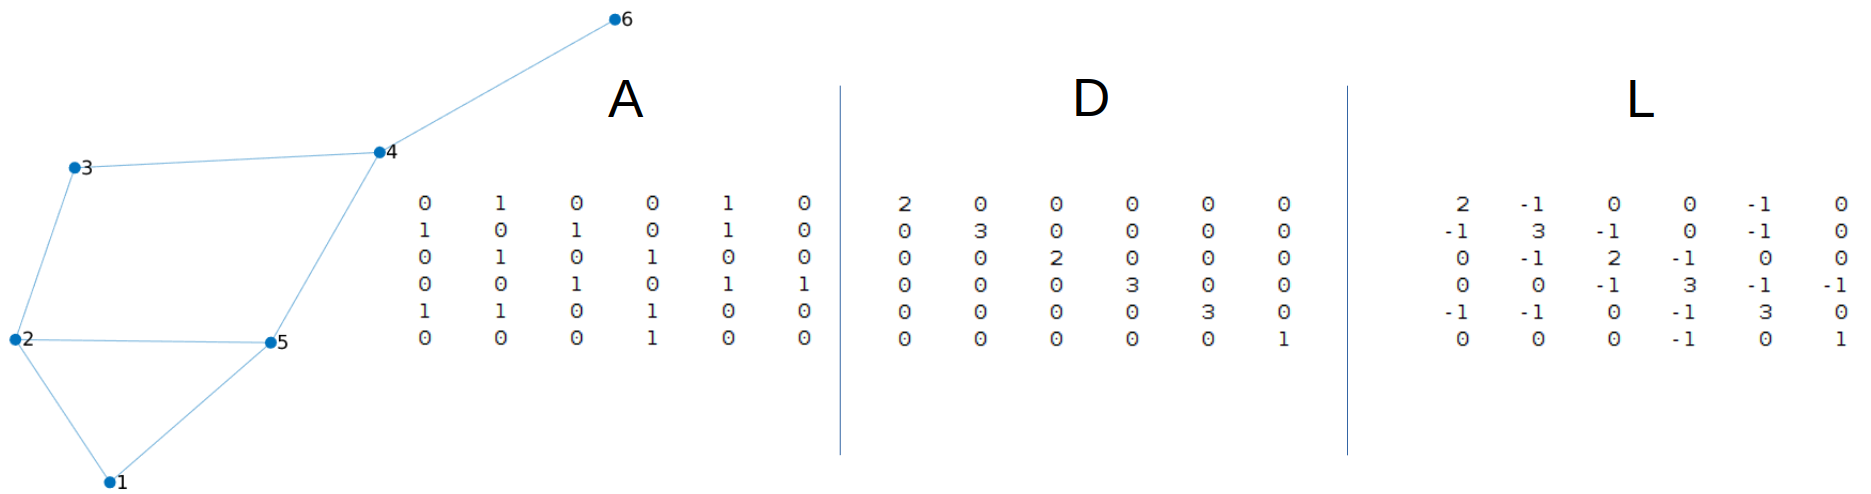
\includegraphics[width=4.8in,height=2.6in]{images/G_A_L.png}
\end{frame}


\begin{frame}{Spectral Clustering Steps}
\begin{itemize}
    \item Calculate similarity matrix A
    \item Calculate Laplacian L
    \item Calculate first k eigenvectors $U_k$
    \item Using $U_k(i,j)$ as embedded feature values, cluster in $\mathbb{R}^k$
\end{itemize}
\end{frame}

\begin{frame}{Variations }
\begin{itemize}
    \item A can be weighted 
    \item Neighbors can be all to nearest k
    \item $L$ can be normalized  $\mathcal{L} = D^{\frac{1}{2}} L D^{\frac{-1}{2}}$
\end{itemize}
\end{frame}


\begin{frame}{X with increasing $p(Class2  ~ Class1)$ }
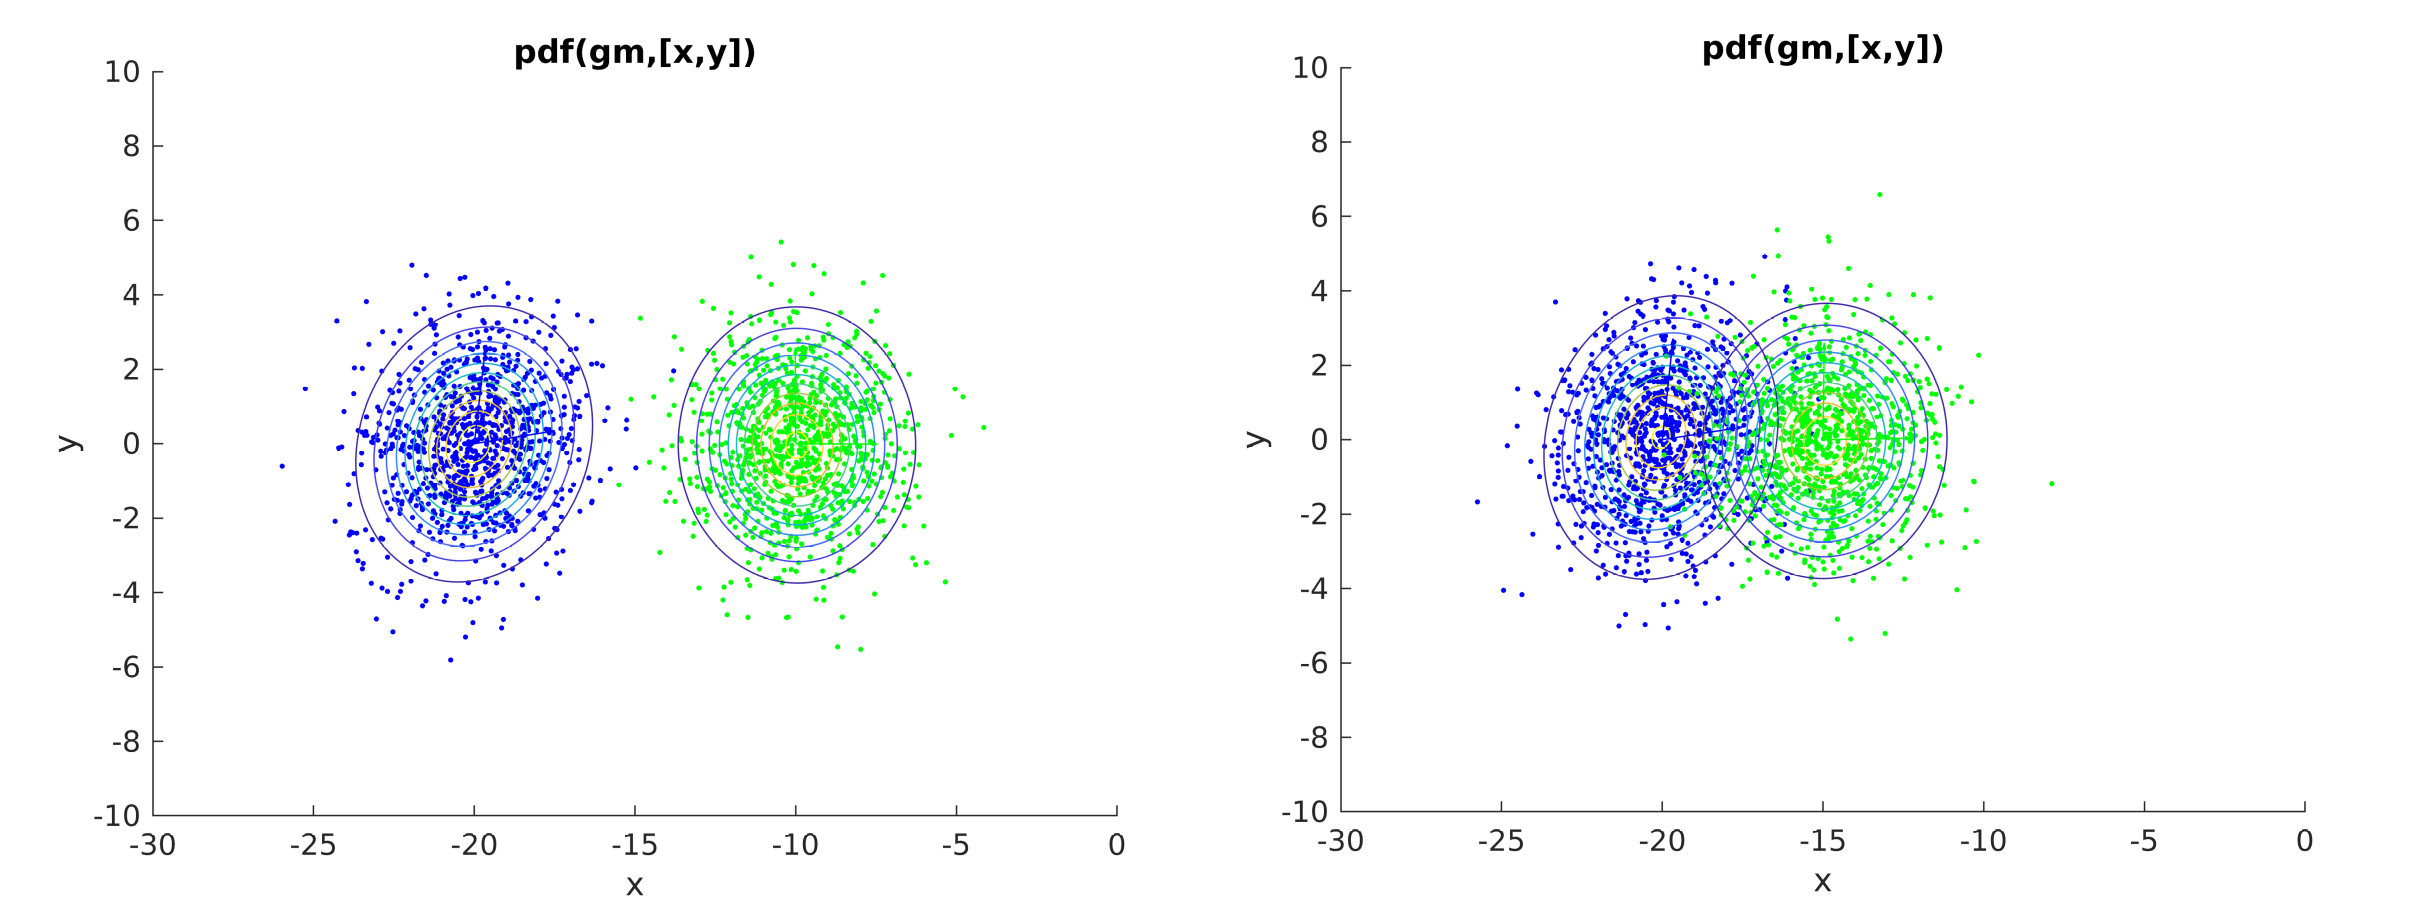
\includegraphics[width=4.8in,height=3.0in]{images/class_dist.png}
\end{frame}


\begin{frame}{A, G with increasing $p(Class2  ~ Class1)$ }
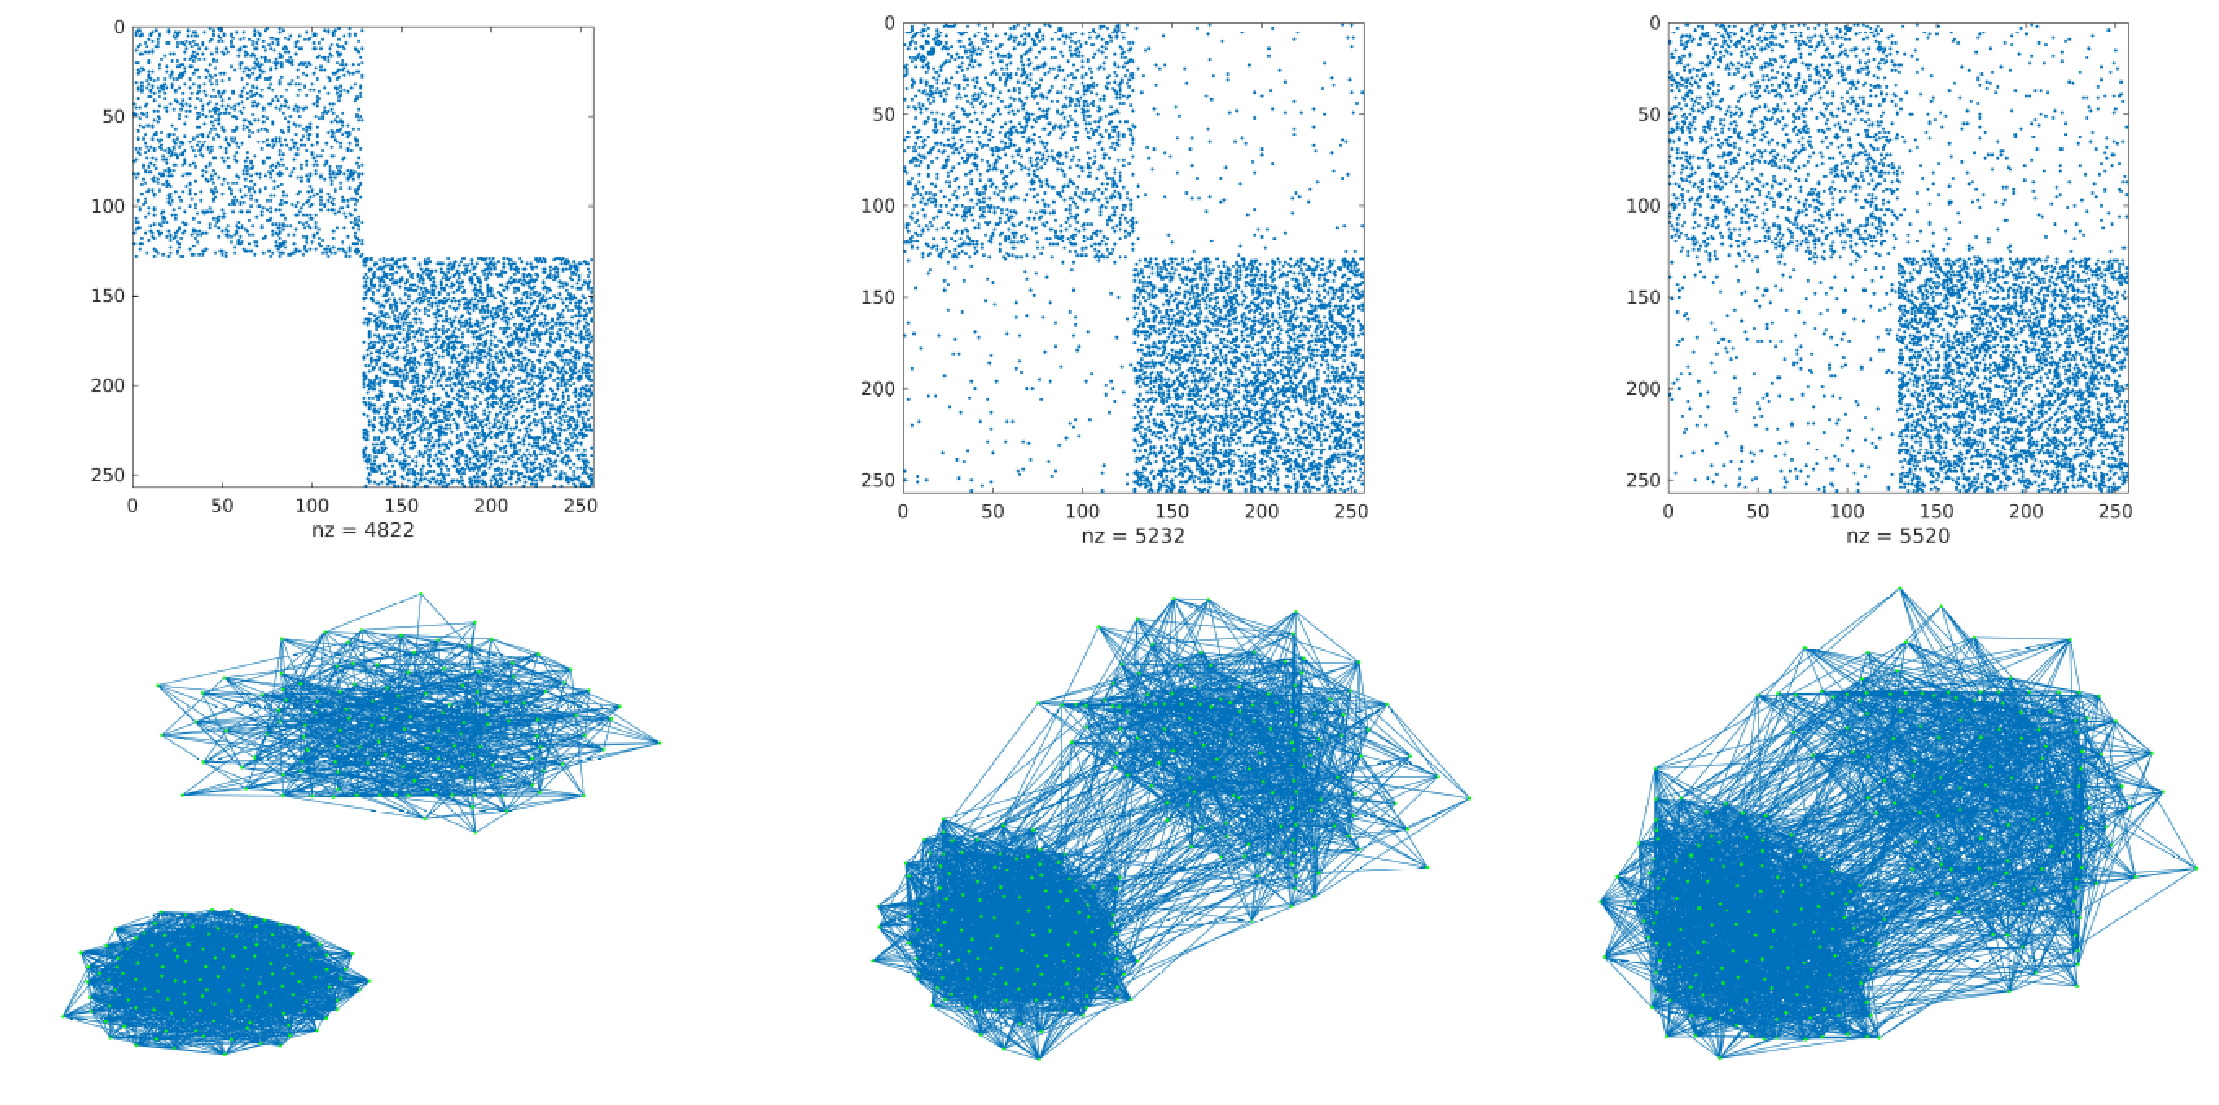
\includegraphics[width=4.8in,height=3.0in]{images/crosstalk.png}
\end{frame}


\begin{frame}{The Spectral Gap}
\begin{itemize}
    \item Cheeger's Inequality - relationship between second eigenvalue and the size of the smallest cut of the graph that separates the classes
    \item We normalize Laplacian because of the close connection to geometry and stochastic processes.  
    \item If we use $\mathcal{L} $ then $D^{-1} A$ is the transition matrix of a random walk on the graph
    \item Close relationship to heat flow problem on a manifold 
\end{itemize}
\end{frame}

\begin{frame}{Spectral Gap with increasing $p(Class2  ~ Class1)$ }
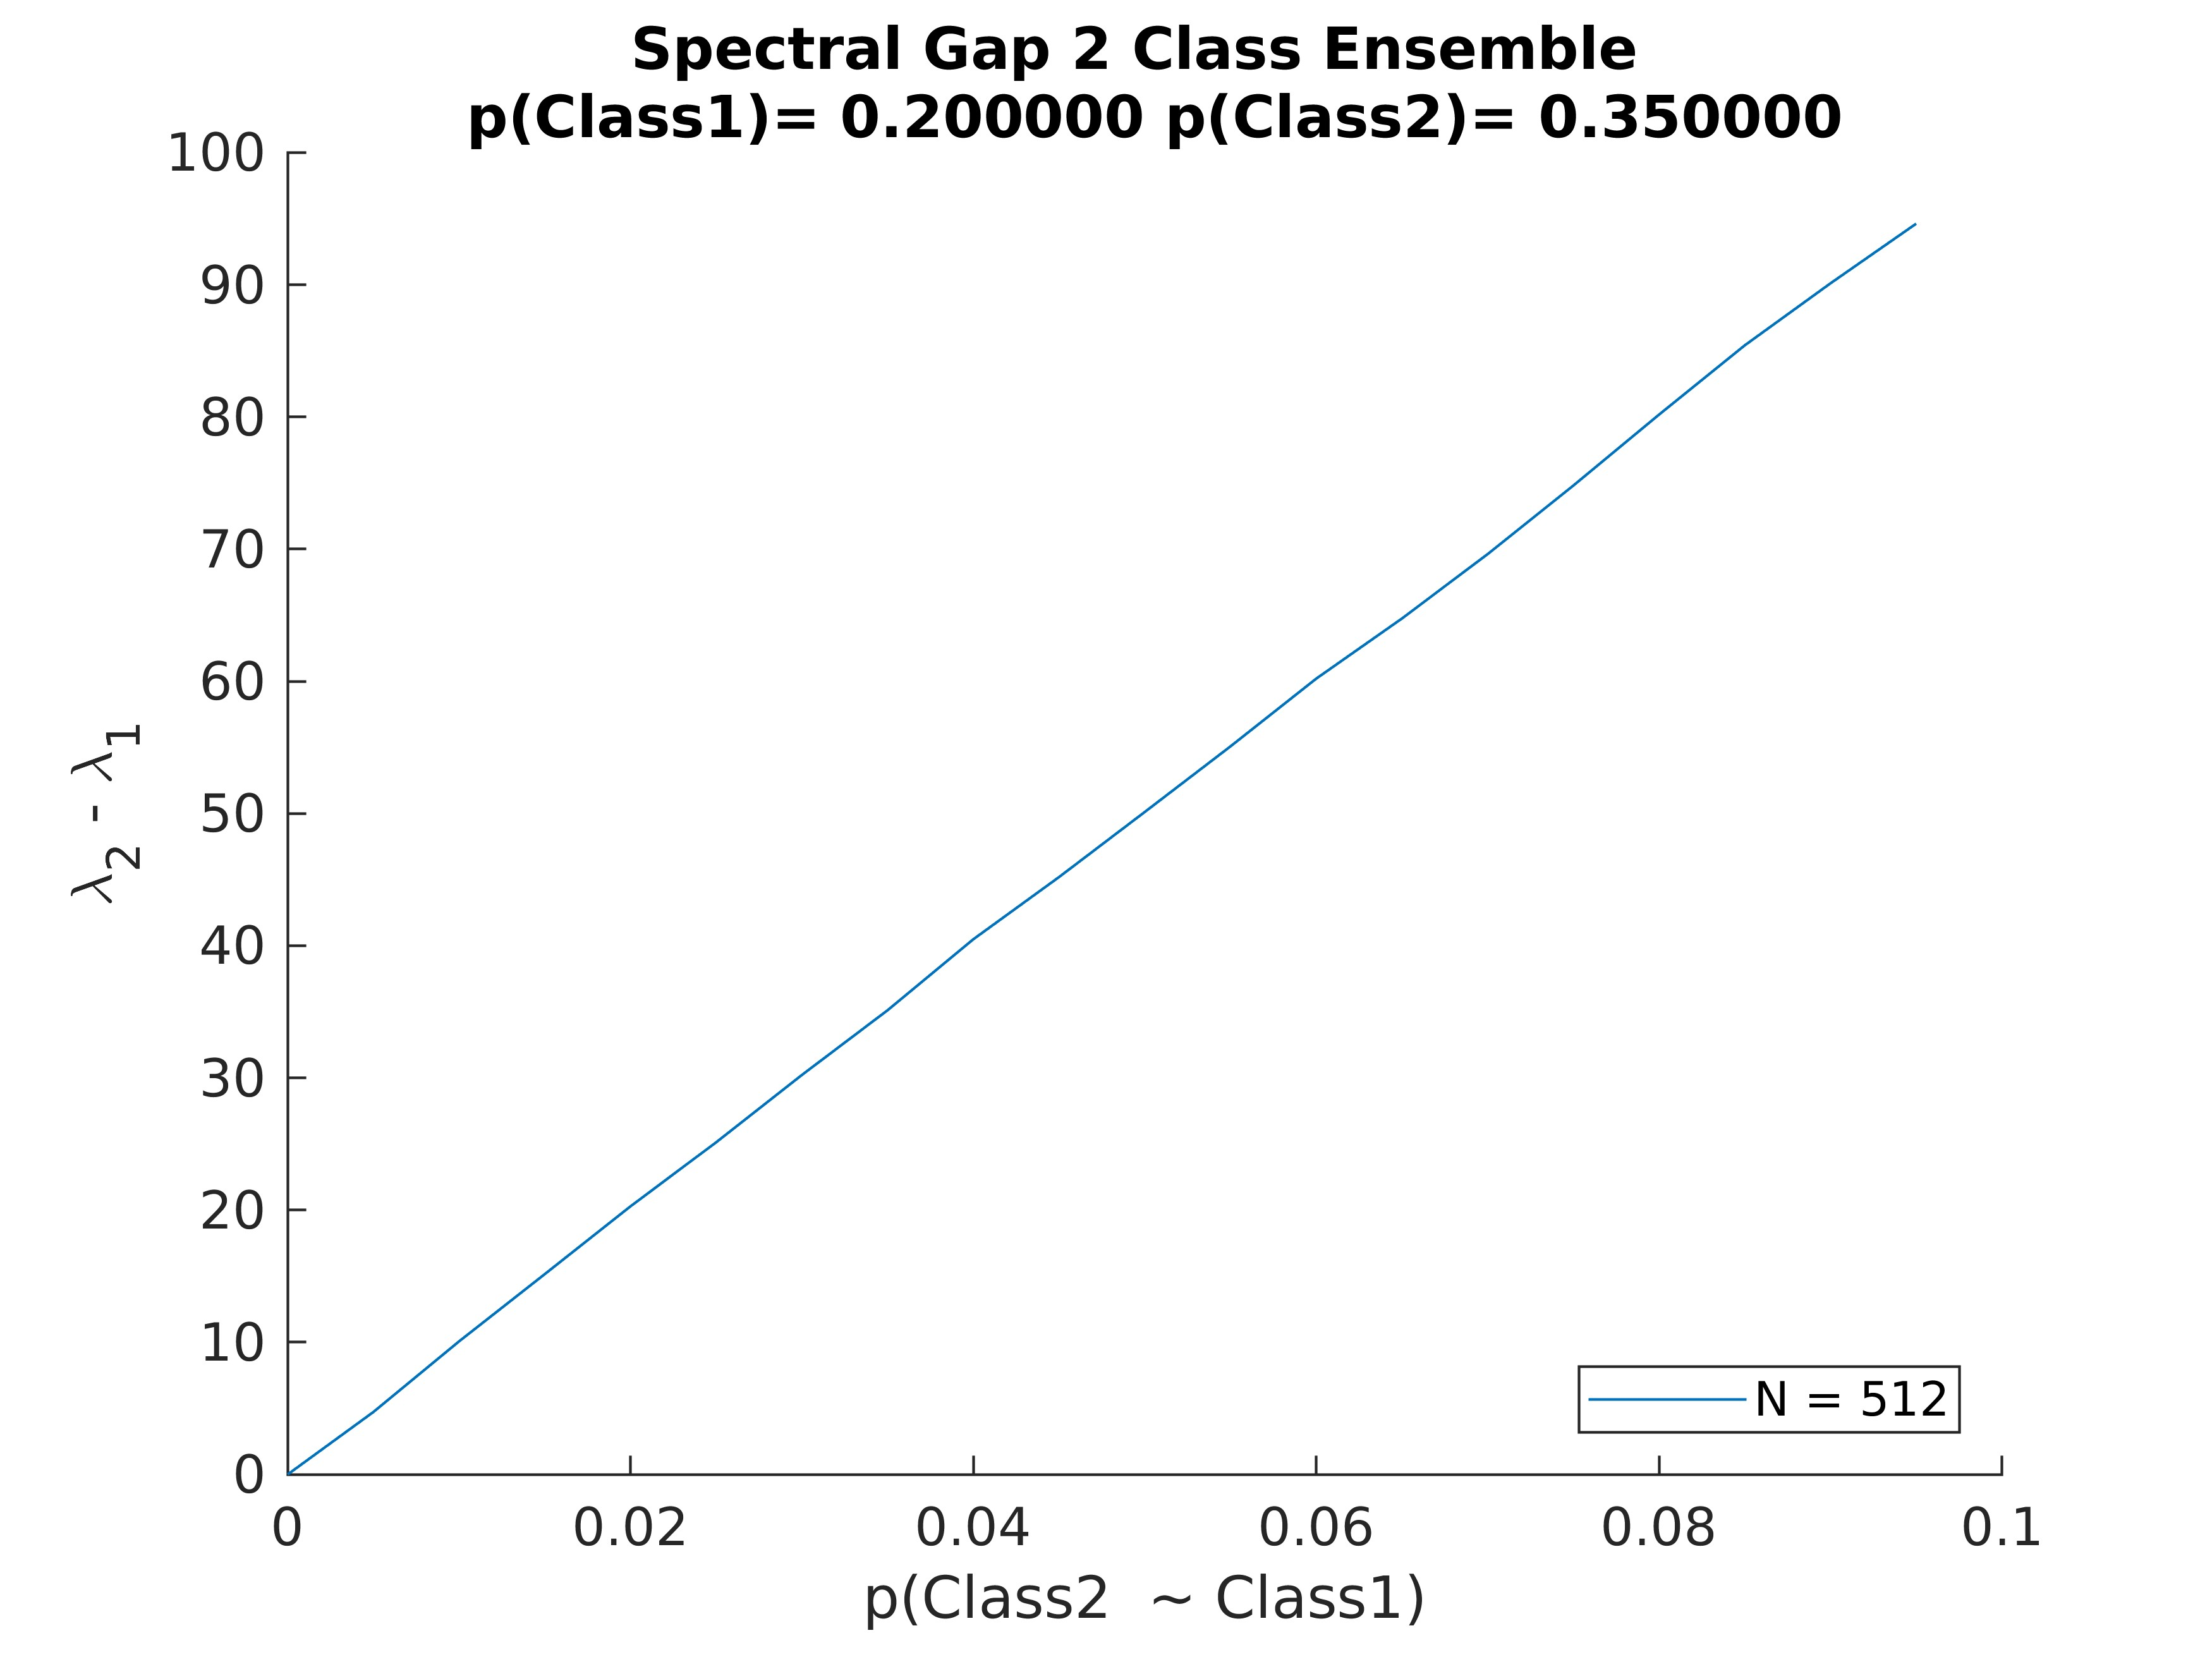
\includegraphics[width=4.8in,height=3.0in]{images/SpectralGap_P1_0.200000P2_0.350000.jpg}
We see Cheeger's inequality  $\lambda_2 \leq \phi(G)$ in action. As crosstalk increases, it becomes harder to partition the data. 
\end{frame}

\begin{frame}{So How Do We Actually Separate The Classes?}
\begin{itemize}
    \item The second eigenvector - the Fiedler Vector - of the graph Laplacian can be considered the first 'fundamental mode' of the graph. 
    \item The spectrum is ordered from lowest to highest values
    \item The eigenvectors are ordered from global to local features. 
    \item We can use the sign of the Fiedler vector to partition
\end{itemize}
\end{frame}

\begin{frame}{Eigenvectors with increasing $p(Class2  ~ Class1)$ }
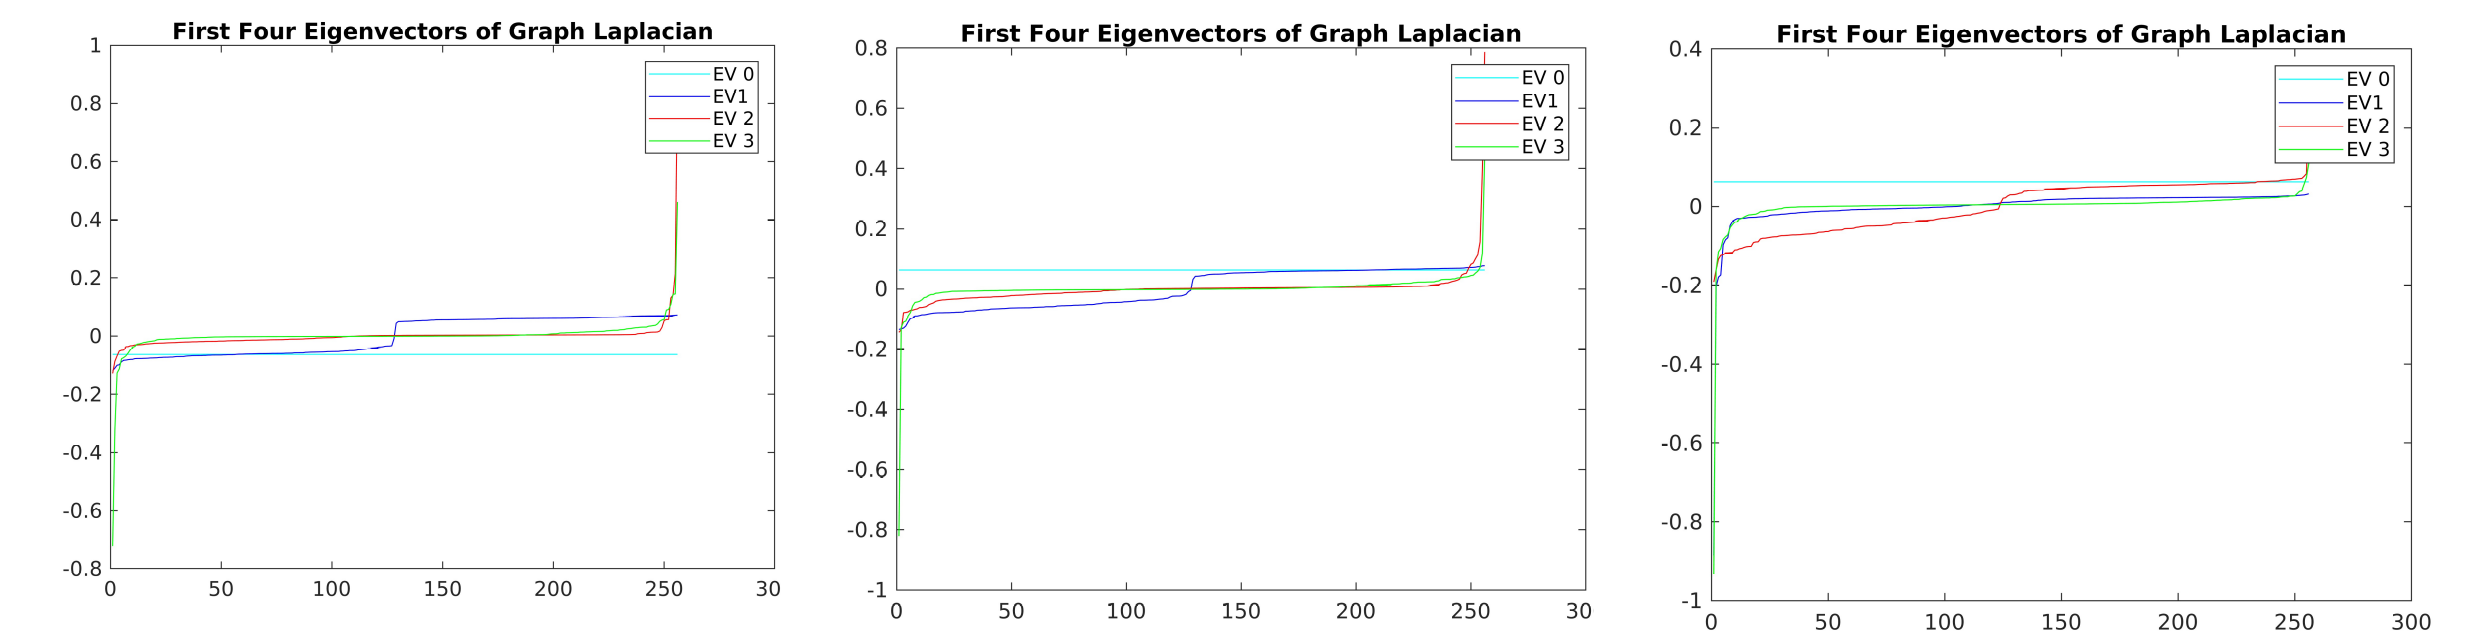
\includegraphics[width=4.8in,height=2.3in]{images/ev4.png}
\end{frame}

\begin{frame}{More Classes }
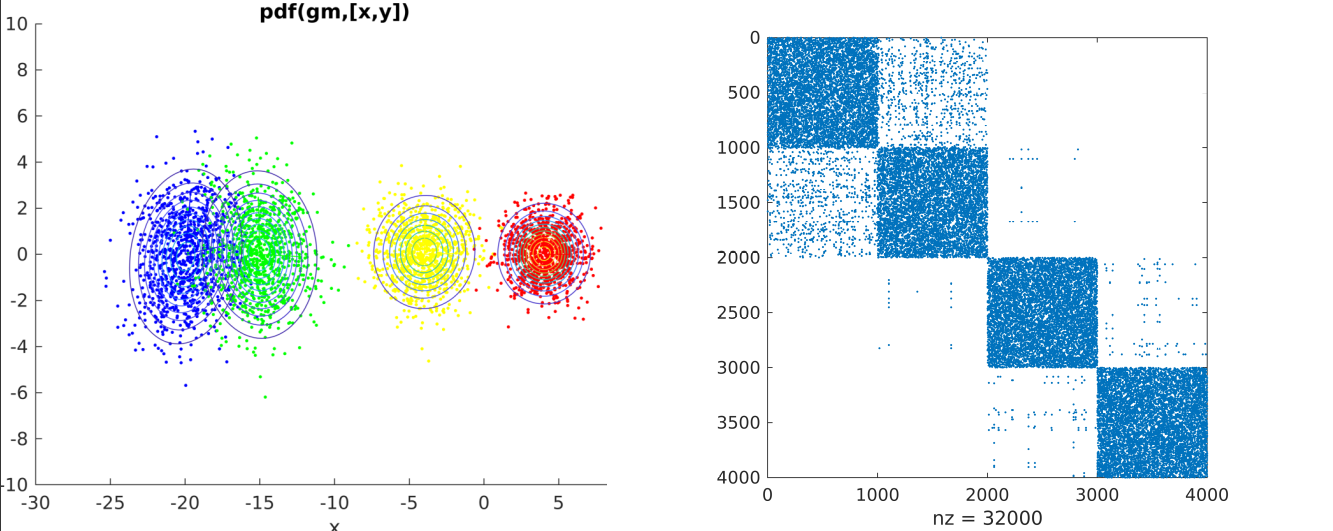
\includegraphics[width=4.3in,height=2.0in]{images/mixed_4.png}
\end{frame}

\begin{frame}{Eigenvectors : 4 Classes }
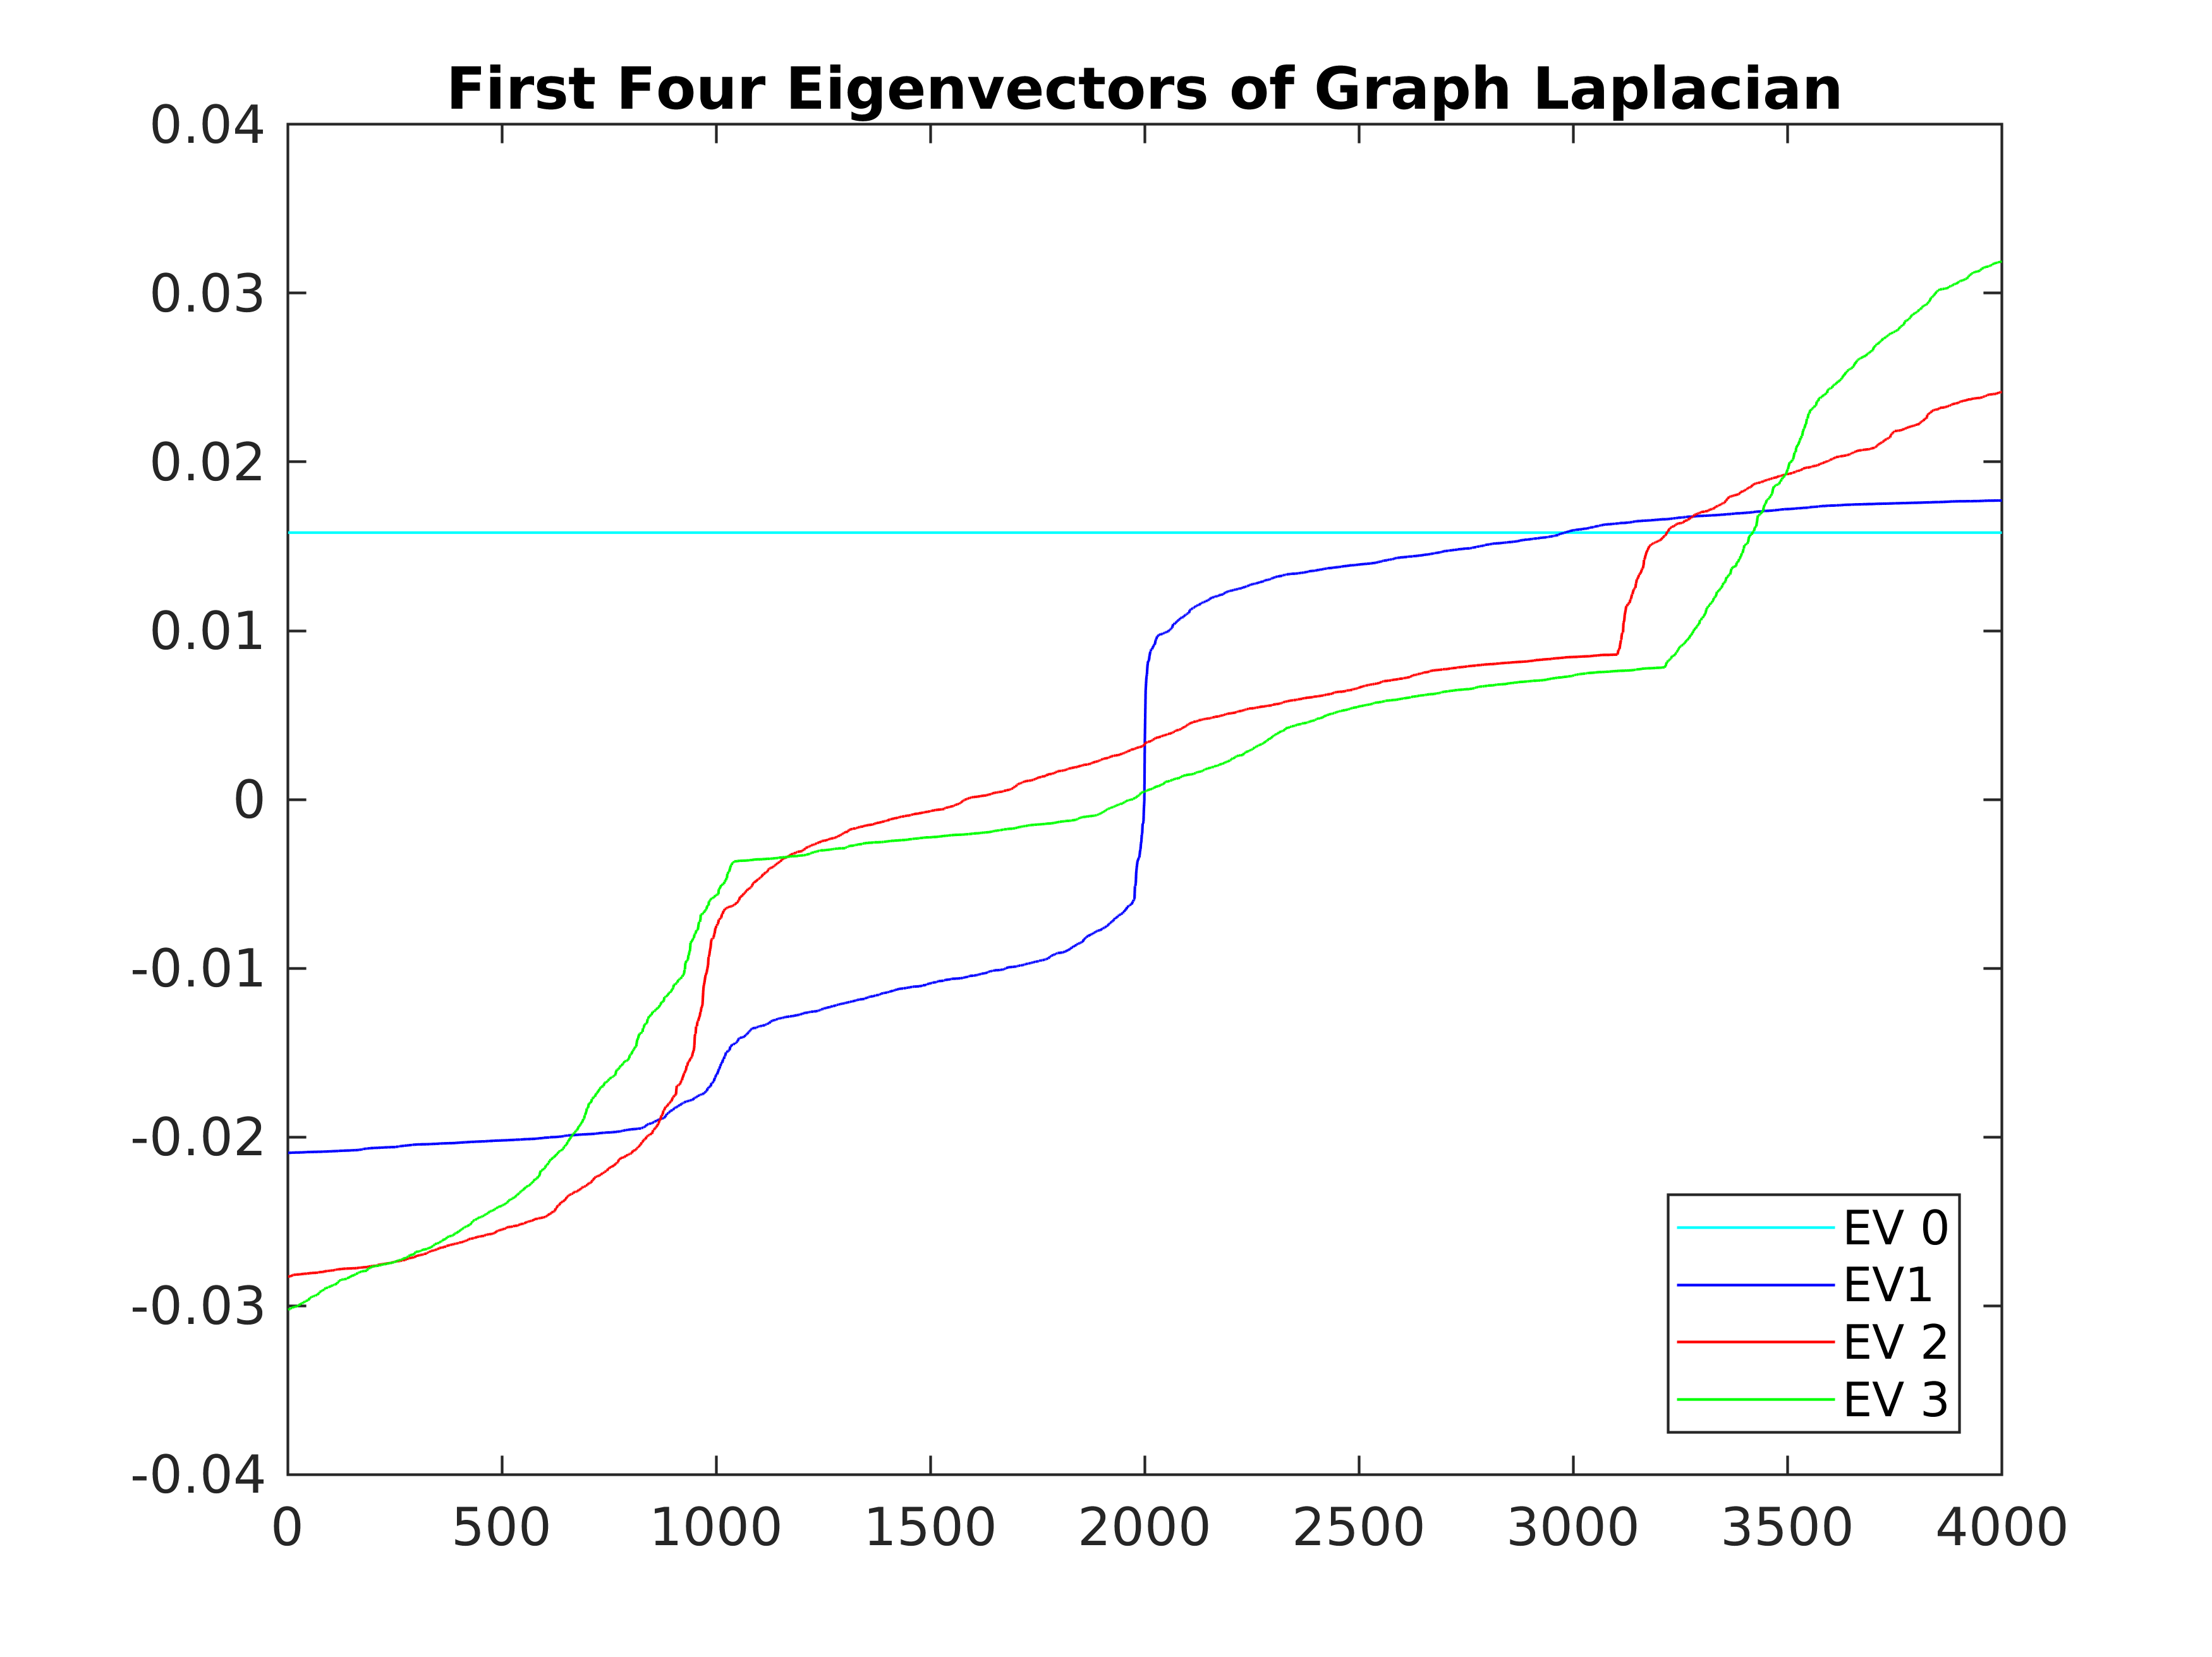
\includegraphics[width=4.2in,height=2.3in]{images/eigenvecs.png}
We notice the eigenvectors associated with non zero eigenvalues all have structure
\end{frame}

\begin{frame}{Blessings and Curses  of High Dimension}
\begin{multicols}
Blessings
\begin{itemize}
\item We may have redundant features - serial correlation in signals etc.
\item Nice theorems about retaining structure after redacting data (Johnson Lindenstrauss )
\end{itemize}
\columnbreak
Curses
\begin{itemize}
\item High dimensional data is sparse
\item The structure we're interested in may be hidden
\item Inference can be difficult due to correlated features and noise dimensions 
\item Counter-intuitive geometry of high dimensional data - most points are orthogonal etc.
\end{itemize}
\end{multicols}
\end{frame}




\begin{frame}{Bibliography}
\begin{thebibliography}{10}
\bibitem{e1}
Spectral Graph Theory, Fan Chung, American Mathematical Soc., 1997

\bibitem{e2}
On Spectral Clustering: Analysis and an algorithm, Ng, Andrew and Jordan, Michael and Weiss, Yair, Advances in Neural Information Processing Systems,2001

\bibitem{e3}
Git Repository, https://github.com/campbell-2589/OSU\_MATH\_5603/tree/main/Project/Report

\end{thebibliography}
\end{frame}


% \begin{frame}[allowframebreaks]
%         \frametitle{References}
%         \bibliography{thebibliography.bib}
% \end{frame}

\end{document}
